\documentclass{beamer}
\usepackage[brazil]{babel}
\usepackage[utf8]{inputenc}

\title{Implementação de Heurísticas em \emph{Prolog} para o Problema do Container}
\author{Bruno Barros Mello, Juliana Moura, Vitor Balestro}
\institute{Universidade Federal Fluminense (UFF)}
\date{\today}

\begin{document}

\begin{frame}
	\titlepage
\end{frame}

\begin{frame}{Conteúdo}
	\tableofcontents
\end{frame}

\section{Introdução e Apresentação do Problema}
\begin{frame}{Introdução e Apresentação do Problema}
	\begin{itemize}
		\item Objetivo: Maximizar o número de caixas empacotadas em um container.
		\item Desafios: Configurações de empacotamento em um espaço tri-dimensional.
		\item Força bruta como benchmark inicial.
		\item Heurísticas abordadas: FFD, FFD com Rotações, LAFF.
	\end{itemize}
\end{frame}

\section{Modelagem do problema}
\begin{frame}{Modelagem do problema}

	\textbf{Variáveis de decisão}
	\begin{itemize}
		\item \texttt{CAIXA(w,h,d)}: conjunto de caixas de dimensões \emph{width}, \emph{height} e \emph{depth}
		\item \texttt{Container(w,h,d)}: container de dimensões \emph{width}, \emph{height} e \emph{depth}
	\end{itemize}

	\vspace{0.5cm}
	\textbf{Função Objetivo}
	\begin{itemize}
		\item Maximizar a quantidade de caixas que cabem em um container
	\end{itemize}

	\vspace{0.5cm}
	\textbf{Restrições}
	\begin{itemize}
		\item Uma caixa não pode colidir com outras caixas no container
		\item Uma caixa deve estar completamente dentro do container
	\end{itemize}
\end{frame}

\section{Representação em prolog}
\begin{frame}{Representação em prolog}

	\begin{itemize}
		\item \textbf{Entrada:} predicados \emph{container} e \emph{box}
		\item \textbf{Entrypoint:} predicado \emph{solve}
		\item \textbf{Estado inicial:} empacotamento vazio
		\item \textbf{Estado final:} empacotamento resultante
		\item \textbf{Mudança de estado:} empacota uma caixa no container
	\end{itemize}
\end{frame}

\section{Benchmark: Força Bruta}
\begin{frame}{Benchmark: Força Bruta}
	\begin{itemize}
		\item Explora todas as combinações possíveis.
		\item Inviável para grandes instâncias devido ao alto custo computacional.
		\item Resultado: Estouro de limite de pilha ao em ambos conjuntos de entrada testados.
	\end{itemize}
\end{frame}

\section{Heurística: First Fit Decreasing}
\begin{frame}{First Fit Decreasing (FFD)}
	\begin{itemize}
		\item Ordena caixas por volume decrescente.
		\item Tenta encaixar cada caixa na primeira posição viável.
		\item Efetivo para maximizar o uso do espaço.
	\end{itemize}
\end{frame}

\section{Heurística: FFD com Rotações}
\begin{frame}{FFD com Rotações}
	\begin{itemize}
		\item Similar ao FFD, mas considera rotações das caixas.
		\item Se uma caixa não cabe, tenta alguma variação de posição.
		\item Melhora o ajuste e eficiência em comparação ao FFD sem rotações.
		\item Resultados mais eficazes para grandes volumes de dados.
	\end{itemize}
\end{frame}

\section{Heurística: Largest Area First Fit (LAFF)}
\begin{frame}{Largest Area First Fit}
	\begin{itemize}
		\item Ordena caixas pela área da base.
		\item Foca na ocupação de superfície.
		\item Menos eficiente em tempo em comparação ao FFD.
	\end{itemize}
\end{frame}

\begin{frame}{Resultados Obtidos (50x50x50)}
	\begin{table}
		\centering

		\resizebox{0.9\linewidth}{!}{
			\begin{tabular}{lcc}
				\textbf{Método}        & \textbf{Caixas Empacotadas} & \textbf{Tempo de Execução} \\
				Força Bruta            & N/A                         & Estouro de Stack Limit     \\
				First Fit Decreasing   & 30                          & 0.338 s                    \\
				FFD com Rotações       & 30                          & 0.160 s                    \\
				Largest Area First Fit & 30                          & 21.911 s
			\end{tabular}
		}
		\caption{Container 50x50x50 com 30 caixas}
	\end{table}
\end{frame}

\begin{frame}{Resultados Obtidos (20x20x20)}
	\begin{table}
		\centering

		\resizebox{0.9\linewidth}{!}{
			\begin{tabular}{lcc}
				\textbf{Método}        & \textbf{Caixas Empacotadas} & \textbf{Tempo de Execução} \\
				Força Bruta            & N/A                         & Estouro de Stack Limit     \\
				First Fit Decreasing   & 10                          & 0.121 s                    \\
				FFD com Rotações       & 10                          & 0.367 s                    \\
				Largest Area First Fit & 10                          & 0.425 s                    \\
			\end{tabular}
		}
		\caption{Container 20x20x20 com 15 caixas}
	\end{table}
\end{frame}

\section{Heurísticas de Custo vs. Avaliação}
\begin{frame}{Heurísticas de Custo}
	\begin{itemize}
		\item As três heurísticas utilizadas — FFD, FFD com Rotação e LAFF — são consideradas heurísticas de custo (passado).
		\item Avaliam o custo imediato ou passado de decisões de empacotamento no contexto atual.
		\item Focam na solução ótima local, sem considerar o custo acumulado de toda a solução.
		\item Diferem das heurísticas de avaliação, que projetam impactos futuros das ações tomadas.
	\end{itemize}
\end{frame}

\section{Dificuldades enfrentadas terminal}
\begin{frame}{Dificuldades enfrentadas}
	\begin{itemize}
		\item Dificuldade para visualizar a solução gerada pelos programas.
		\item Utilizamos o jogo \textit{Minecraft} para contornar esta limitação
	\end{itemize}

	\begin{figure}
		\centering
		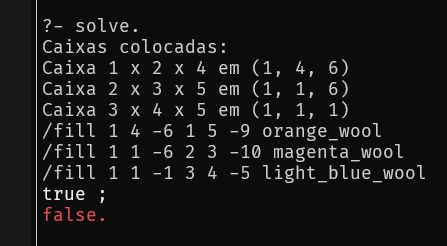
\includegraphics[width=0.8\textwidth]{minecraft-terminal.jpg}
		\caption{Comandos para gerar blocos no minecraft}
	\end{figure}
\end{frame}

\section{Dificuldades enfrentadas jogo}
\begin{frame}{Dificuldades enfrentadas}
	\begin{itemize}
		\item Dificuldade para visualizar a solução gerada pelos programas.
		\item Utilizamos o jogo \textit{Minecraft} para contornar esta limitação
	\end{itemize}

	\begin{figure}
		\centering
		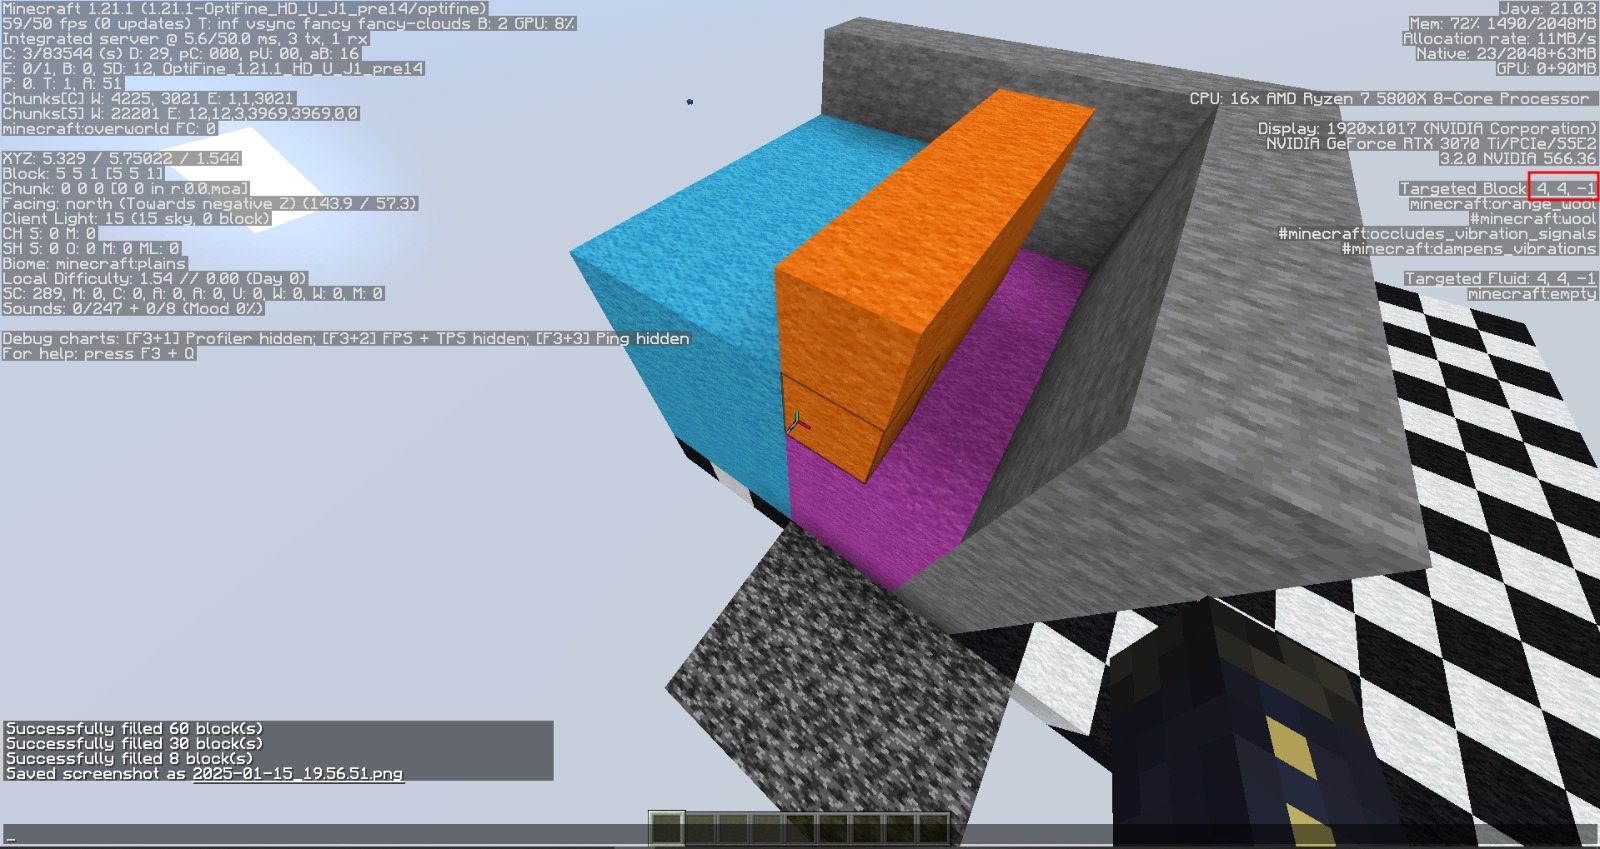
\includegraphics[width=0.8\textwidth]{minecraft-jogo.jpg}
		\caption{Comandos para gerar blocos no minecraft}
	\end{figure}
\end{frame}

\section{Conclusões}
\begin{frame}{Conclusões}
	\begin{itemize}
		\item Métodos baseados em volume são geralmente mais eficientes.
		\item Consideração de rotações melhora resultados.
		\item LAFF, apesar de atingir bons resultados para entradas menores, tem performance prejudicada exponencialmente para entradas maiores.
		\item Força bruta é impraticável exceto para pequenos casos.
	\end{itemize}
\end{frame}

\end{document}
